\documentclass[11pt]{article}

\usepackage[margin=1in, letterpaper]{geometry}
\usepackage{parskip}
\usepackage{amsthm, amsmath, amssymb}
\usepackage{enumerate} % For use of (a), (b), et cetera
\usepackage[pdftex]{graphicx}
\usepackage{hyperref}

% The following metadata will show up in the PDF properties
\hypersetup{
    colorlinks = true,
    urlcolor = black,
    pdfauthor = {Aaron Tran},
    pdfkeywords = {berkeley},
    pdftitle = {Astro 121, UG Radio Lab, Lab 1 - \today},
%   pdfsubject = {},
    pdfpagemode = UseNone
}

% Don't indent paragraphs
\setlength\parindent{0em}

% Problem numbering
\newcounter{iternum}
\setcounter{iternum}{0}
\newcommand{\prob}{\stepcounter{iternum} \textbf{\arabic{iternum}.} }
\newcommand{\probcont}{\textbf{\arabic{iternum}. (cont.) }}

% ===============
% Useful commands
% ===============
\newcommand {\mt}{\mathrm}
\newcommand {\unit}[1]{\; \mt{#1}}
% http://vemod.net/typesetting-units-in-latex

% ==========================
% Document specific commands
% ==========================

\begin{document}

% Titling
\begin{center}
\Large{Design and construction of a $1.045 \unit{MHz}$ FM receiver}

\large
Aaron Tran \\
\today \\
Partners: Patrick Kantorski, Kyle Moses \\
Prof. Aaron Parsons, GSI Karto Keating, uGSI Baylee Bordwell
\end{center}

\section*{\sffamily Abstract}

Karto's general rule: one sent. for each sect.
Give numbers (e.g., transmission line speed)

\section{Introduction}

Modulation of radio frequency (RF) electromagnetic waves is a simple and
effective method for long distance information transmission, as exemplified by
amplitude/frequency modulated radio.  The generation, transmission, and
reception of modulated signals are interesting engineering problems which are
also accessible to interested amateurs and beginning students of electronics.
Simple modulators and demodulators may be built with a minimum
of passive and active components (i.e., enough to fit on a small breadboard).
RF circuits hold great educational potential for undergraduate students.

Here we present the design and construction of an FM receiver ($1.045
\unit{MHz}$ with bandwidth $200 \unit{kHz}$).  The only non-linear components
necessary are a diode and a transistor.  The primary purpose of this circuit is for self-edification, but the layout may also serve as a starting point for
further exploration of RF circuit design.

Additional paragraphs on results

\section{FM receiver design}

The receiver is comprised of a passive RLC bandpass filter, diode envelope
detector, and a common-emitter amplifier chained between antenna input and
speaker output.  Blocking capacitors are placed between different functional
sections to enable voltage biasing.

\begin{figure}[h]
    \centering
    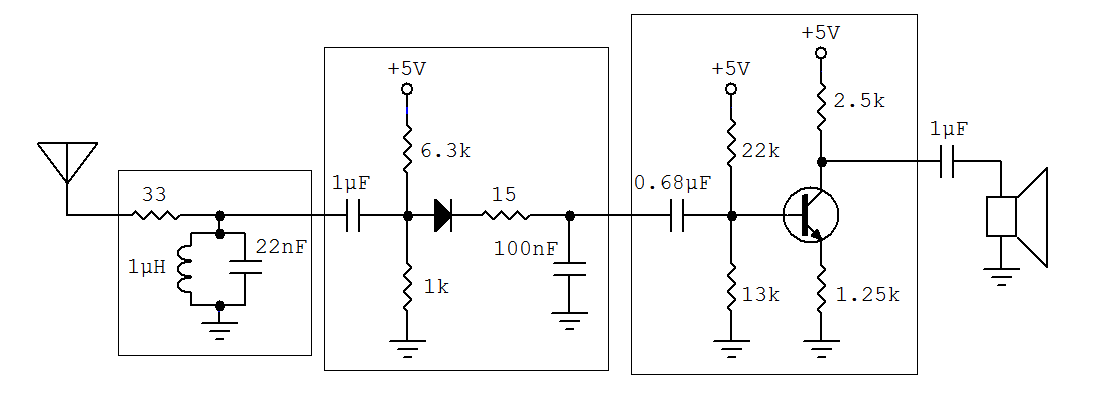
\includegraphics[scale=0.5]{schematics/receiver_box.png} \\
    \textbf{Figure 1.} FM receiver circuit diagram with component values. Boxes
    demarcate functional components (see corresponding sections in text).
\end{figure}

\subsection{Bandpass RLC filter}

The input signal is first passed through an RLC filter centered at
approximately $1.045 MHz$ with the $-3 \unit{dB}$ point at $\pm 200 \unit{kHz}$
on each side.  For component values $R, L, C$ (resistor, inductor, capacitor)
and input signal component with angular frequency $\omega$, the gain of this
filter is given by the equation:
\[
  \left| \frac{V_{\mt{out}}}{V_{\mt{in}}} \right| =
    \left(
      1 + (RC)^2 \left(\frac{\omega_0^2 - \omega^2}{\omega}\right)^2
    \right)^{-1/2}
\]
Here $\omega_0 \equiv 1 / \sqrt{LC}$, emphasizing that this filter has unity
gain at $\omega = \omega_0$.  The $-3 \unit{dB}$ roll-off frequency occurs
when the gain is equal to $1/\sqrt{2}$,or when:
\[
  (RC) \frac{\omega_0^2-\omega^2}{\omega} = 1
\]
Let the bandwidth be denoted by $\Delta f$, with corresponding cut-offs at
$f = f_0 \pm \Delta f /2$, where $f_0 = w_0/(2\pi)$.  This gives:
\[
  2 \pi f_0 RC \approx \frac{f_0}{\Delta f}
\]
as a prescription for our cut-off.  Our component values $R = 33 \unit{\Omega},
L = 1 \unit{\mu H}, C = 22 \unit{nF}$ (Figure 1) give $f_0 = 1.073 \unit{MHz}$,
with bandwidth $\Delta f = 220 \unit{kHz}$.  Figure 2 plots the
frequency-dependent gain along with the transmission band of interest at $1.045
\unit{MHz}$.

\begin{figure}[h]
    \centering
    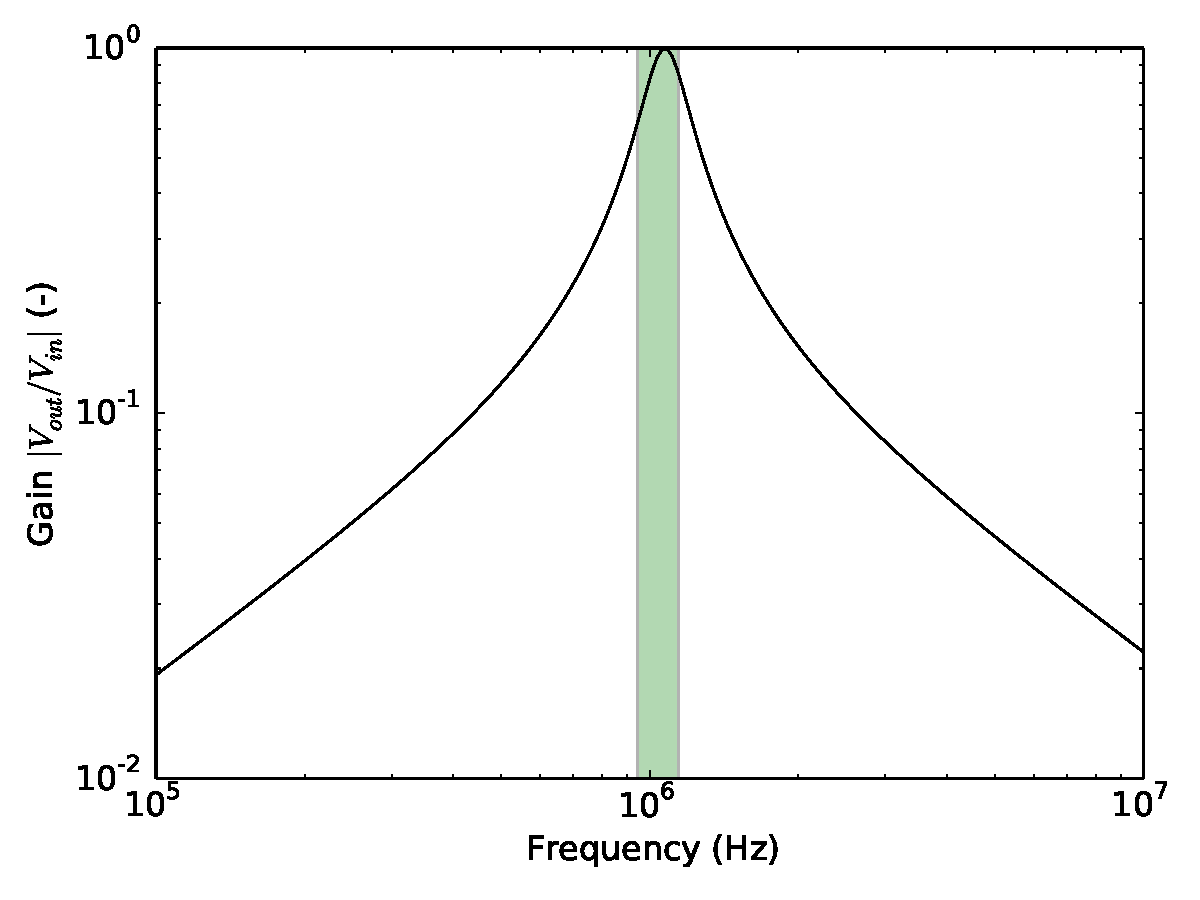
\includegraphics[scale=0.5]{scripts/rlc_filter_gain.pdf} \\
    \textbf{Figure 2.} RLC filter gain as a function of input frequency $f$
    (Hz).  FM signal bandwidth plotted in light green.
\end{figure}



\subsection{Diode envelope detector}

* Describe overall design of receiver, with subsections for each functional plot.  List salient features for each (-3dB point, bias voltages @ various locations, etc.). Present as if you invented it, and are writing a seminal paper (hahahaha)

* Plot expected output of LC filter in receiver as function of $f$.  Mark transmission band on plot and explain rationale behind its placement on response curve.

* Plot bandpass of final filter that defines band of output audio signal.  Describe (maybe plot) rationale for selecting said filter.

\subsection{Common-emitter amplifier}

* Describe speaker amplifier (circuit diagram), describe how it works, parts, bias voltages.  Define operating band - what frequency range, and what sets the bounds?

* Suppose speaker amplifier connects to speaker at end of long wire.  Given the circuit we built, what impedance cable do you recommend, how to terminate it (with 8-ohm speaker) to avoid reflections?  Don't worry about maximizing current through speaker.

* Specify input/output impedance of circuit at audio frequencies



\section{Results}

* Discuss transmission line results.

\subsection{Demodulator debugging}

To test the RLC bandpass filter, we input a sine wave of varying frequencies
and measured the output across the $LC$ tank circuit.  We obtained a maximum
gain of $0.83$ at input frequency $1.05 \unit{MHz}$ (caveat: we may have used
incorrect termination procedure for this measurement, but this only impacts our
measurement of gain).  The circuit qualitatively showed the correct roll-off
behavior.  When we input an FM signal at $1.045 \unit{MHz}$ and observed the
filter output on an oscilloscope, the signal was correctly converted into
an AM signal with envelope code matching output audio.

* Explain our odd troubles with the diode detector.  Whether the circuit helped was very equivocal...

\subsection{Amplifier tests}

* Discuss frequency / clipping issues here?

\subsection{Noise characterization}

* Noise measurement

\section{Discussion}

* Amplifier test - explain Allan variance test, but give reasonable physical numbers

\section{Conclusion}

What you're gonna do with this next.  Don't rewrite your intro/abstract.

Use plain english.  Don't worry about being technical, or too concise...

\section{Acknowledgments}

Circuit diagrams were generated using Fritzing.

\section{References}

\end{document}
